\chapter{State of the art}
\label{ch:marco}

\section{Realated work}

Most of the work related to the detection of diseases and pests in tomato make use of deep learning techniques, but specifically the supervised learning algorithms. In \cite{Fuentes2017_2} is presented work of the use of CNN classifiers and object detectors like Faster R-CNN, Region-based Fully Convolutional Network or Single Shot Multibox Detector for the detections of disease in tomato in South Korea. One of the problems that this project faced was the false positives,  in \cite{Fuentes2018} is proposed a filter to reduce this issue.

In \cite{AsimeniaDimokranitou2017} propose the use of an adversarial autoencoder for anomaly detection. This corresponds to an unsupervised method that is just able to replicate healthy data. This method has the advantage that the network is able to find the main features that represent normal data.

In \cite{Baur2019} presents a new architecture proposal where is combined the variational autoencoder and the generative adversarial networks, for the detection of anomalies in MR brain images. This new architecture is compared with other approaches like general VAE, spatial VAE, and AnoGAN. The authors claim that its VAEGAN architecture slightly outperforms most of the other architectures.

\section{Literature review}

\subsection{Deep Feedforward Networks}

The Deep Feedforward Networks, also known as multilayer perceptrons (MLPs), has a big importance in the field of Machine Learning. The problem that this kind of network tackle is the approximation of some function \begin{math} f^{*}\end{math}. As mentioned in \cite{goodfellow_bengio_courville_2017}, a common example is in the implementation of a classifier where \begin{math} y = f^{*}(x)\end{math} maps the input \begin{math} x \end{math} to some category represented in \begin{math} y \end{math}. In order to achieve that the feedforward networks define a mapping of the form \begin{math} Y = f(X, \theta)\end{math}, and during the training, this network should be able to learn the set of parameters \begin{math} \theta \end{math} that best fits to approximate the function.

These networks are typically composed of many different functions, which represent the layers of the network. For example, we could have four functions that are connected in cascade, to the form \begin{math} f(x) = f_{(4)}(f_{(3)}(f_{(2)}(f_{(1)}(x)))) \end{math}. The length of these chains of functions can be seen as the depth of the network, where \begin{math} f_{(1)} \end{math} is the first layer and \begin{math} f_{(4)} \end{math} is the last layer of the output. Between the first and the output layers are the hidden layers. During the training, generally is provided explicitly the output values given some input, but is no specified what values should have the hidden layers. The learning algorithm should decide how to use those hidden layers to generate the desired output.

\subsection{Convolutional Neural networks}

The convolutional neural networks (CNN) \cite{Lecun1999} are an extension of the deep feedforward networks, that are specialized in the processing of grid-like data. As its name suggests, this kind of network makes use of a mathematical operation called convolution. The convolution is an operation on two functions of a real-valued argument and is defined as follows:

\begin{equation}
 s(t)=\int x(a) w(t-a) d a
\end{equation}

In terms of CNN, the first argument of the convolution (\begin{math} x(a) \end{math}) is referred as the input and the second argument (\begin{math} w(t - a) \end{math}) as the kernel. The output of this operation is known as the feature map. The common architecture of a CNN, as shown in figure \ref{fig:cnn}, is composed of a convolutional layer, then a pooling layer (which is in charge of subsampling the data) and in the end, there is typically a fully connected network.

\begin{figure}[htb]
  \centering
  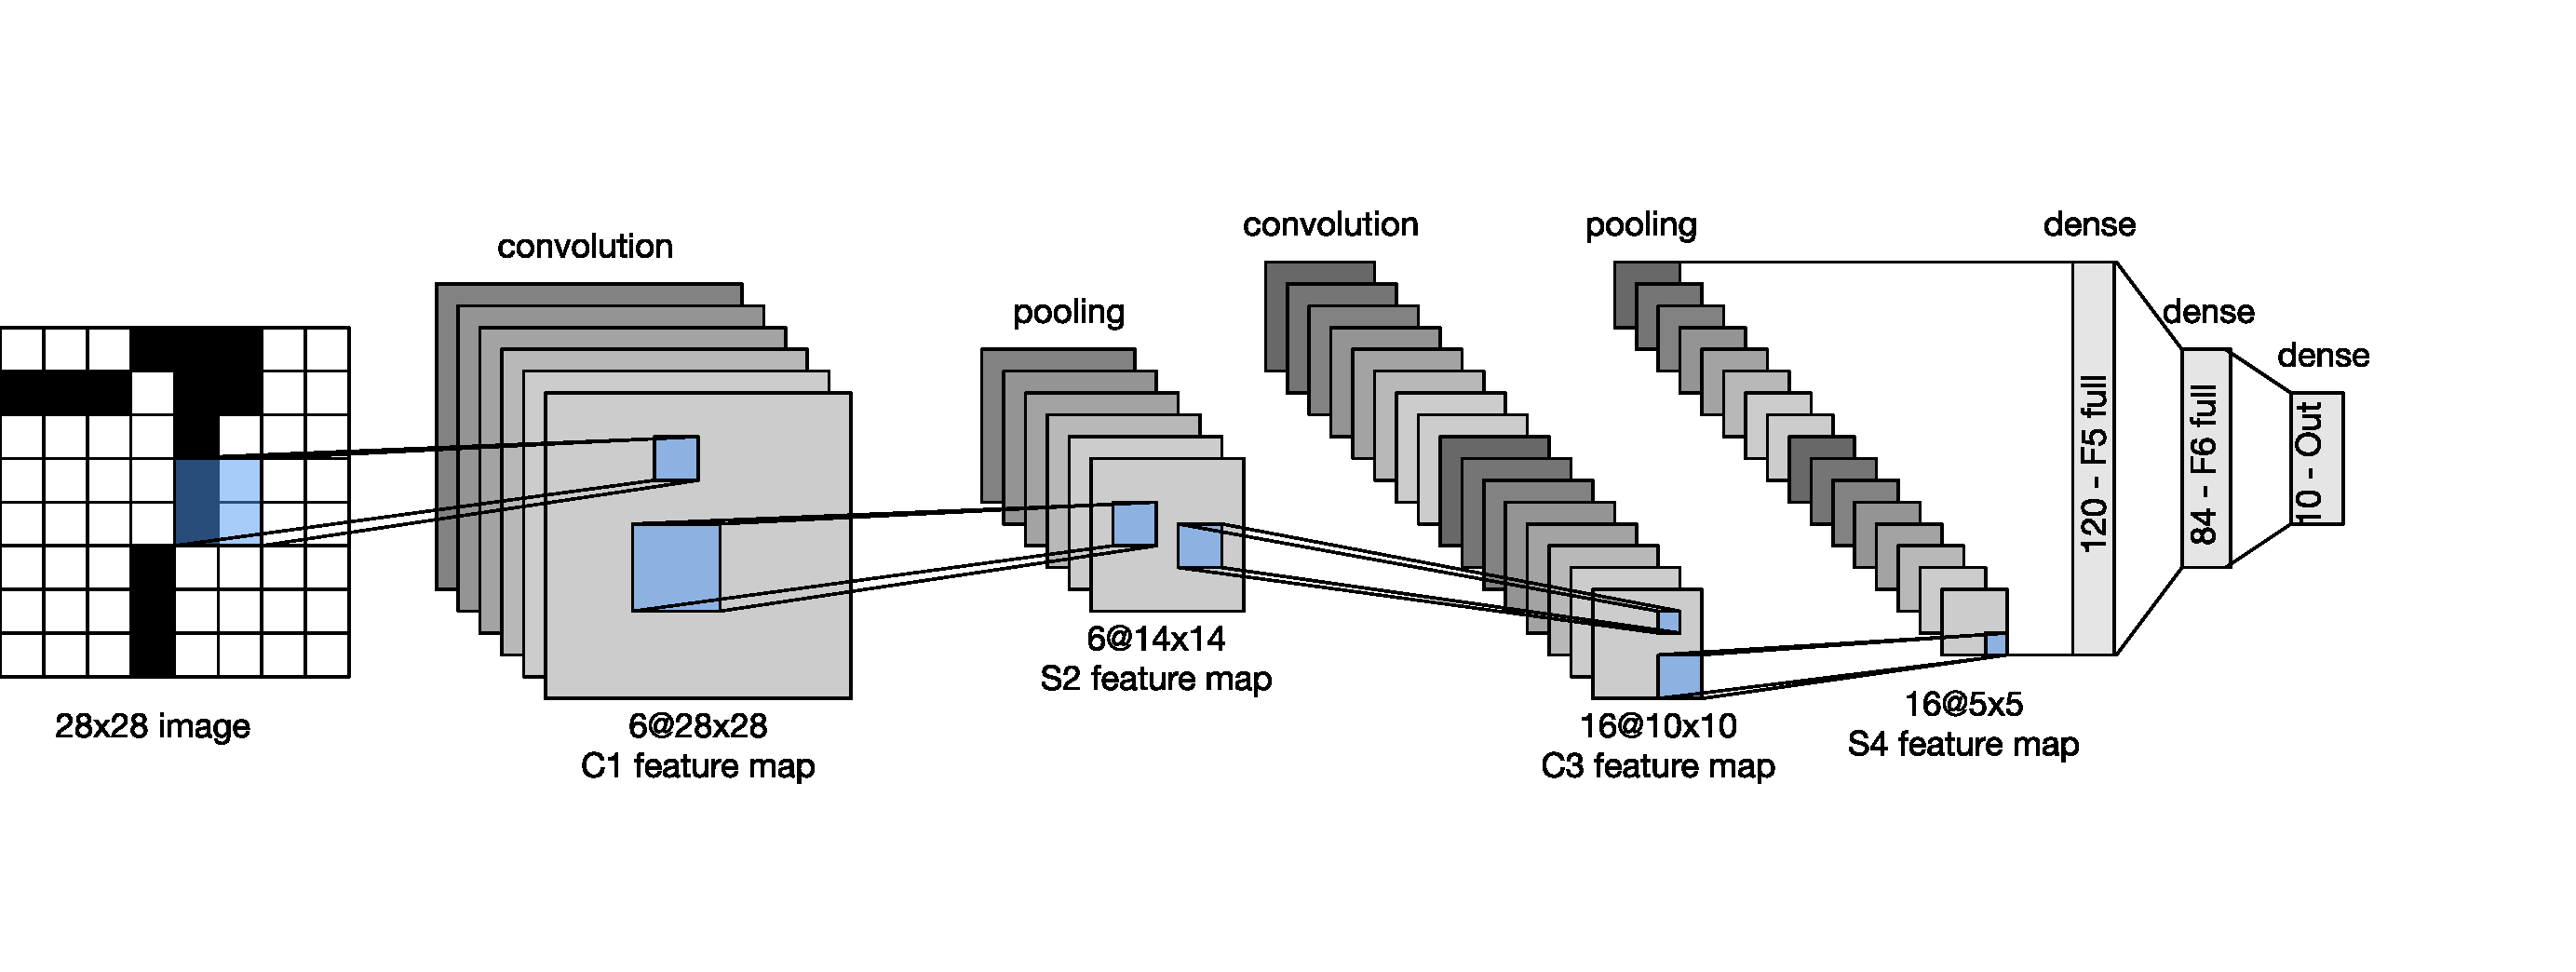
\includegraphics[width=150mm]{CNN}
  \caption[Convolutional Neural Network architecture]{Convolutional Neural Network architecture}
  \label{fig:cnn}
\end{figure}

\subsection{Generative models}

In machine learning, there are mainly three types of learning algorithms: supervised learning algorithms, unsupervised learning algorithms, and semi-supervised learning algorithms. The supervised learning algorithms are the type of algorithms that make use of labeled data for its training process. In the last years, this kind of algorithm is presenting very important results in applications like object detection \cite{Liu2019}.

The unsupervised learning algorithms are the ones that do not need a structured dataset and can find a pattern by itself. One particular type of unsupervised learning algorithms is the generative models. The generative models are powerful algorithms that are capable of learning the probabilistic data distribution of some datasets, allowing them to generate new samples. Two of the most important generative models are the variational autoencoders (VAE) and the generative adversarial networks (GAN).

\subsubsection{Autoencoders}

In a similar way as the CNNs, the autoencoders are an extension of the deep feedforward network, with the difference that in this case, the goal is to replicate the input in the output. This type of networks are divided into two parts: the encoder that tries to generate a latent space h where is extracted some features of the input data \begin{math} h = f(x) \end{math}; and the decoder that takes the latent space generated by the encoder as input and reconstruct the data \begin{math} r = g(h) \end{math}. One of the main applications of the type of neural networks is the dimensionality reduction, image compression, image denoising or image generation. The last application example shall be cover in more detail in the next section with the variational autoencoders as part of the generative models.

\begin{figure}[htb]
  \centering
  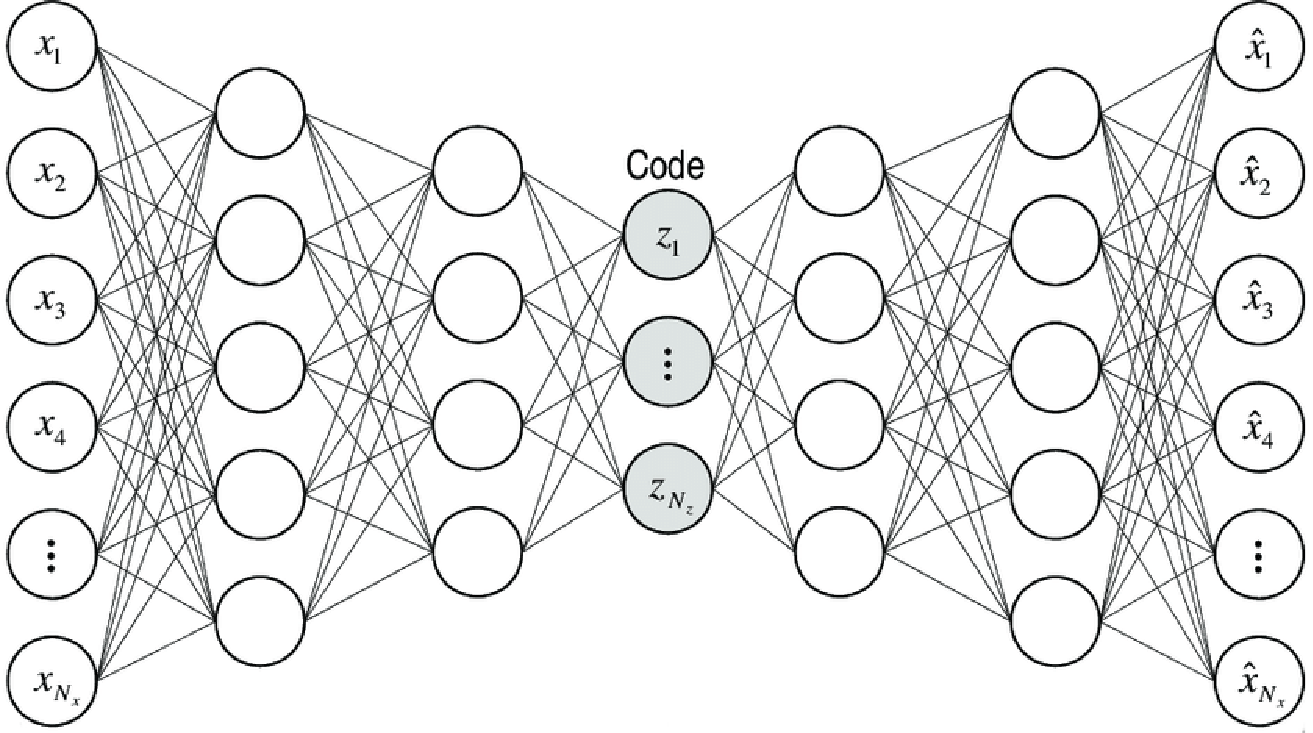
\includegraphics[width=80mm]{autoencoder}
  \caption[Autoencoder architecture]{Autoencoder architecture}
  \label{fig:autoencoder}
\end{figure}

\textit{Variational Autoencoder}

The objective of the variational autoencoders \cite{Kingma2014} is the generation of data samples from a learned latent space. This latent space is obtained from a large dataset. In order to achieve this generation process, this autoencoders must try to learn the probability distribution \begin{math} P(x) \end{math} of the data.

From a probabilistic perspective, the latent variables will get from a prior \begin{math} P(z) \end{math} and the generated data has a likelihood of \begin{math} P(X|z) \end{math} that is conditioned by the latent space. So the goal here is to model de data distribution as follows:

\begin{equation}
 \mathbb{P}(\mathbf{X})=\int_{z} \mathbb{P}(\mathbf{X} | z) \mathbb{P}(z) d z
\end{equation}

However, this integral is computationally too costly, due to the fact of computing all the possibilities in the latent space. To avoid this, VAEs tries to infer the distribution \begin{math} \mathbb{P}( x ) \end{math} from data using \begin{math}\mathbb{P}(z|\mathbb{X})\end{math}. Variational inference approximates the distribution \begin{math}\mathbb{P}(z | \mathbb{X})\end{math}, using a simpler distribution, where a common choice is a Gaussian distribution. Then, with a parametric inference model \begin{math}\mathbb{Q}(z|\mathbb{X})\end{math} that maps the input data with the latent space; the difference between the distribution \begin{math}\mathbb{P}(z|\mathbb{X})\end{math} and \begin{math}\mathbb{Q}(z|\mathbb{X})\end{math} is calculated using the Kullback-Leibler divergence.

\begin{equation}
 \begin{aligned} D_{K L}(\mathbb{Q}(z | \mathbf{X}) \| \mathbb{P}(z | \mathbf{X})) &=\sum \mathbb{Q}(z | \mathbf{X}) \log \frac{\mathbb{Q}(z | \mathbf{X})}{\mathbb{P}(z | \mathbf{X})} \\ &=\mathbb{E}\left[\log \frac{\mathbb{Q}(z | \mathbf{X})}{\mathbb{P}(z | \mathbf{X})}\right] \\ &=\mathbb{E}[\log \mathbb{Q}(z | \mathbf{X})-\log \mathbb{P}(z | \mathbf{X})] \end{aligned}
 \label{eq:dkl}
\end{equation}

Using \begin{math}\mathbb{P}(z | \mathbf{X})=\frac{\mathbb{P}(\mathbf{X} | z) \mathbb{P}(z)}{\mathbb{P}(\mathbf{X})}\end{math}, the equation \ref{eq:dkl} can be rewritten as:

\begin{equation}
 \begin{aligned} D_{K L}(\mathbb{Q}(z | \mathbf{X}) \| \mathbb{P}(z | \mathbf{X})) &=\mathbb{E}\left[\log \mathbb{Q}(z | \mathbf{X})-\log \frac{\mathbb{P}(\mathbf{X} | z) \mathbb{P}(z)}{\mathbb{P}(\mathbf{X})}\right] \\ &=\mathbb{E}[\log \mathbb{Q}(z | \mathbf{X})-\log \mathbb{P}(\mathbf{X} | z)-\log \mathbb{P}(z)+\log \mathbb{P}(\mathbf{X})] \end{aligned}
\end{equation}

\begin{math}\mathbb{P}(x)\end{math} does not depend on \begin{math}z\end{math}, hence it can be taken out of the expectation:

\begin{equation}
 \begin{aligned} \Longrightarrow \log \mathbb{P}(\mathbf{X})-D_{KL}(\mathbb{Q}(z | \mathbf{X}) \| \mathbb{P}(z | \mathbf{X})) &=\mathbb{E}[\log \mathbb{P}(\mathbf{X} | z)]-\mathbb{E}[\log \mathbb{Q}(z | \mathbf{X})-\mathbb{P}(z)] \\ &=\mathbb{E}[\log \mathbb{P}(\mathbf{X} | z)]-D_{KL}(\mathbb{Q}(z | \mathbf{X}) \| \mathbb{P}(z)) \end{aligned}
\end{equation}

Therefore, the loss function corresponds to:

\begin{equation}
 \log \mathbb{P}(\mathbf{X}) \geq \mathbb{E}[\log \mathbb{P}(\mathbf{X} | z)]-D_{KL}(\mathbb{Q}(z | \mathbf{X}) \| \mathbb{P}(z))
\end{equation}

The first term of the loss function can be seen as the reconstruction error and the second term corresponds to the KL error \cite{Doersch2016}.

\textit{Spatial Variational Autoencoder}

Consist of an improvement of the typical variational autoencoder. Whereas in the classic VAEs the latent space are vectors where its variables have a dimension of 1x1, in the spatial VAE the idea is to extend these latent variables to have a bigger dimension and, in that way, be able to capture more spatial features of the input data.

In \cite{Wang2019} is proposes a spatial variational autoencoder, where the latent variables are sampled from a matrix-variable normal (MVN) distribution. The authors claim that this architecture outperforms the original VAEs due to the capture of richer structural and spatial information from data.

\textit{Gaussian-Mixure Variational Autoencoder}

This architecture corresponds to another variant of the VAEs models. In this case, the prior distribution \begin{math}\mathbb{P}(z)\end{math} is a Gaussian-mixture that allows the net to perform unsupervised clustering of the data. This autoencoder, proposed in \cite{Dilokthanakul2016}, has the potential of group the data, and each group can represent or share a specific feature of the original data, besides to have a competitive performance in comparison with the regular VAEs.

\subsubsection{Generative adversarial networks}

The generative adversarial networks (GAN) were proposed by Ian Goodfellow \cite{Goodfellow2014} in 2014. The basic idea behind GANs is in the competence of two models: from one side is the generator G that tries to learn the data distribution of the data and for the other side, a discriminator \begin{math}\mathbb{D}\end{math} that decides if the input data is real or generated by \begin{math}\mathbb{G}\end{math}. The goal of the generator is to try to create images as real as possible that provokes the discriminator to make mistakes.  This game is described as the minmax value function in equation \ref{eq:gan}.

\begin{equation}
 \min _{G} \max _{D} V(D, G)=\mathbb{E}_{x \sim p_{\text {data }}(x)}[\log D(x)]+\mathbb{E}_{z \sim p_{z}(z)}[\log (1-D(G(z)))]
 \label{eq:gan}
\end{equation}

A well trained GAN model is able to reach the Nash equilibrium, where the discriminator has an accuracy of around 0.5, which means that it is not able to discern between fake or real data; and the generator should reach value loss of approximately 0.7.

\begin{figure}[htb]
  \centering
  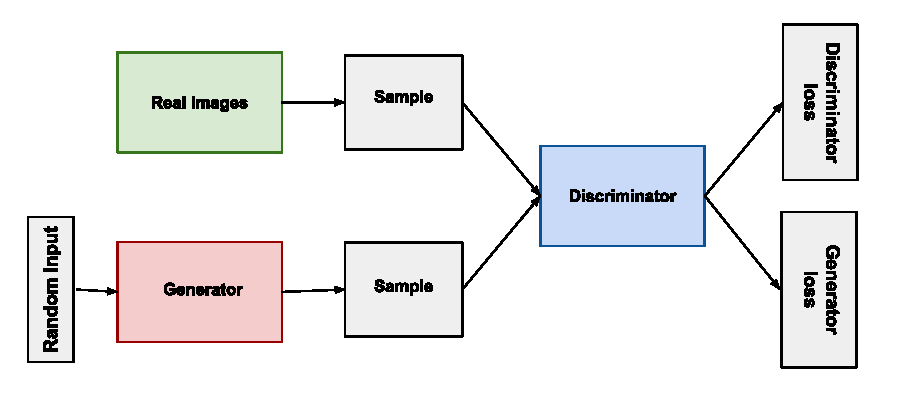
\includegraphics[width=120mm]{gan_diagram}
  \caption[Generative Adversarial Network architecture]{Generative Adversarial Network architecture}
  \label{fig:gan}
\end{figure}

One of the major challenges that the GANs has is precisely the training process, where something is really hard to reach the Nash equilibrium. Sometimes, if the capacity of the model is not enough, the model is susceptible to collapse. Another possible scenario is when the learning rate of the model is too aggressive, provoking that the model never converges.

\textit{Architectures based on GANs}

In \cite{Pan2019} presents a series of architectures based on GANs, along with some metrics to evaluate its performance.

\begin{itemize}
 \item \underline{Convolution base GAN}: The original GAN is implemented based on the multi-layer perceptron but it has been proven that CNN are better than the MLP in extracting features to the images. This kind of network is known as Deep Convolutional Generative Adversarial Network (DCGAN).
 \item \underline{Conditional GAN}: Normally, the generator of the GAN receives as input some random noise, which sometimes makes the model prone to collapse. It is for this reason that in the conditional GAN a variable C is introduced as input to the generator and also to the discriminator, with the objective of add some constraints and, therefore, have more control in that latent space. The type of constraint will depend on the type of data that the GAN is dealing with.
 \item \underline{Autoencoders based GANs}: This type of GAN architecture is presented in \cite{Makhzani2015} where the idea is to make use of an adversarial training to the autoencoder performing variational inference by matching the aggregated posterior latent space of the autoencoder with an arbitrary prior distribution. This will allow overcoming one of the main challenges of the autoencoders, where sometimes is not able to learn correctly the data distribution.
\end{itemize}

\subsection{Use of generative model in the anomaly detection}

The generative models discussed so far have their utility in the detection of anomalies. The general idea is to train a model to be able to learn the data distribution of a normal dataset. In that way, the model should be able to reconstruct o generate a query image as similar as possible. If for some reason that is not the case, there is a high probability that the regions that the model was not able to generate, correspond to an anomaly. All the autoencoders described before can be used in this way, as well as the GANs.

For the specific case of the GANs, in \cite{DiMattia2019} is presented different GAN based architectured, with the propose of anomaly detection:

\subsubsection{AnoGAN}

This GAN is first trained with just normal data and be able to learn the manifold of the data X. Then, with the generator trained, each time that some image has to be evaluated, an iterative process is performed in order to find the latent variables that generate the more similar \begin{math}G(x)\end{math} to the query image. This iterative process has the disadvantage that is too time-consuming \cite{Schlegl2017}.

\begin{figure}[htb]
  \centering
  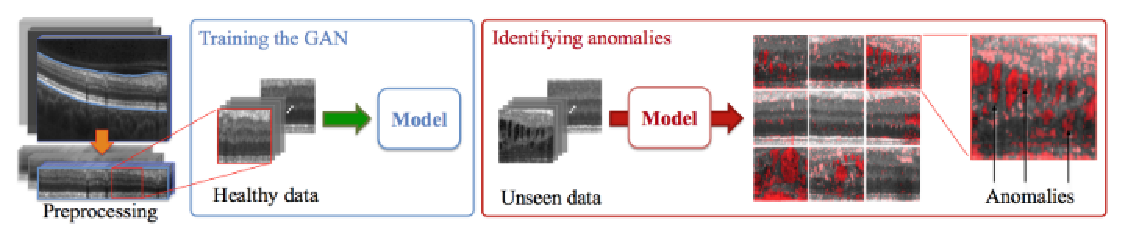
\includegraphics[width=150mm]{anogan}
  \caption[AnoGAN]{AnoGAN traing with healty images first and then reconstruction of unseen images\cite{Schlegl2017}}
  \label{fig:anogan}
\end{figure}

\subsubsection{GANomaly}

This architecture is inspired by the AnoGan but tries to overcome the long detection time that it has. In order to do that, make use of an encoder that is able to learn the latent space variables that the generator receives during the GAN training. This has the advantage of having a faster GAN training and reduces the times to generate a similar image to the query image. The generator also has an encoder at the end of its structure that helps in the training in the learning of the manifold of the input data x.

\begin{figure}[htb]
  \centering
  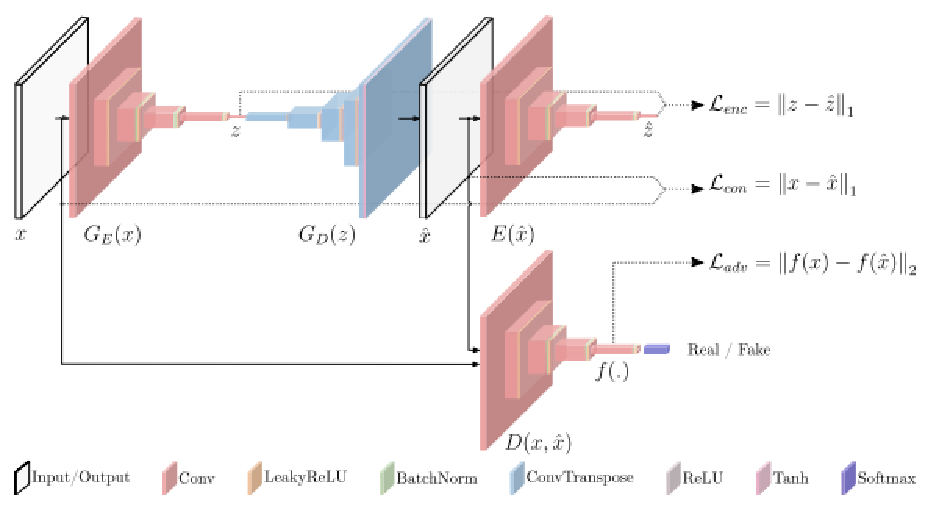
\includegraphics[width=130mm]{ganomaly}
  \caption[GANomaly]{GANomaly architecture and loss functions \cite{DiMattia2019}}
  \label{fig:ganomaly}
\end{figure}
